\chapter{LHC ATLAS実験}
本章では,\ref{sec:LHC}節でLHC加速器について述べ,\ref{sec:ATLAS-ex}節でATLAS実験について,また,\ref{sec:ATLAS}節でATLAS検出器について述べる.そののち,\ref{sec:HL-LHC}節でHigh Luminosity LHC計画について説明し,それに伴うATLAS検出器アップグレードについて説明する.\par
\section{LHC加速器}
\label{sec:LHC}
Large Hadron Collider(LHC)はスイス、ジュネーブにある欧州原子核研究機構(CERN)の地下100 $\mathrm{m}$,周長26.7 $\mathrm{km}$のリングで構成される円形加速器である.最大で14TeVの重心系エネルギーで陽子陽子衝突させることが可能な,世界最大の陽子陽子衝突型加速器である.新粒子の探索や,ヒッグス粒子やトップクォーク等の質量が大きい粒子を多く生成できるので,結合定数などの精密測定も行うことが可能である.LHCには,陽子・陽子衝突点を4点設けていて,各衝突点に,衝突に伴う生成粒子の観測を目的として,大型の検出器(ATLAS, ALICE, CMS, LHCb)が配置されている.2015-2018年にかけて陽子ビームのエネルギーが6.5 $\mathrm{TeV}$,重心系衝突エネルギーでは13 $\mathrm{TeV}$,瞬間ルミノシティは$2\times 10^{34} \mathrm{cm^{-2}s^{-1}}$で物理実験が行われている.図\ref{fig:LHC}にLHC加速器の全体図を示す.LHCでは,陽子はバンチという塊で連なりビームを形成し,25 $\mathrm{ns}$に1回,すなわち40 $\mathrm{MHz}$でバンチ同士の衝突が行われている.\par

\begin{figure}[h]
  \centering
  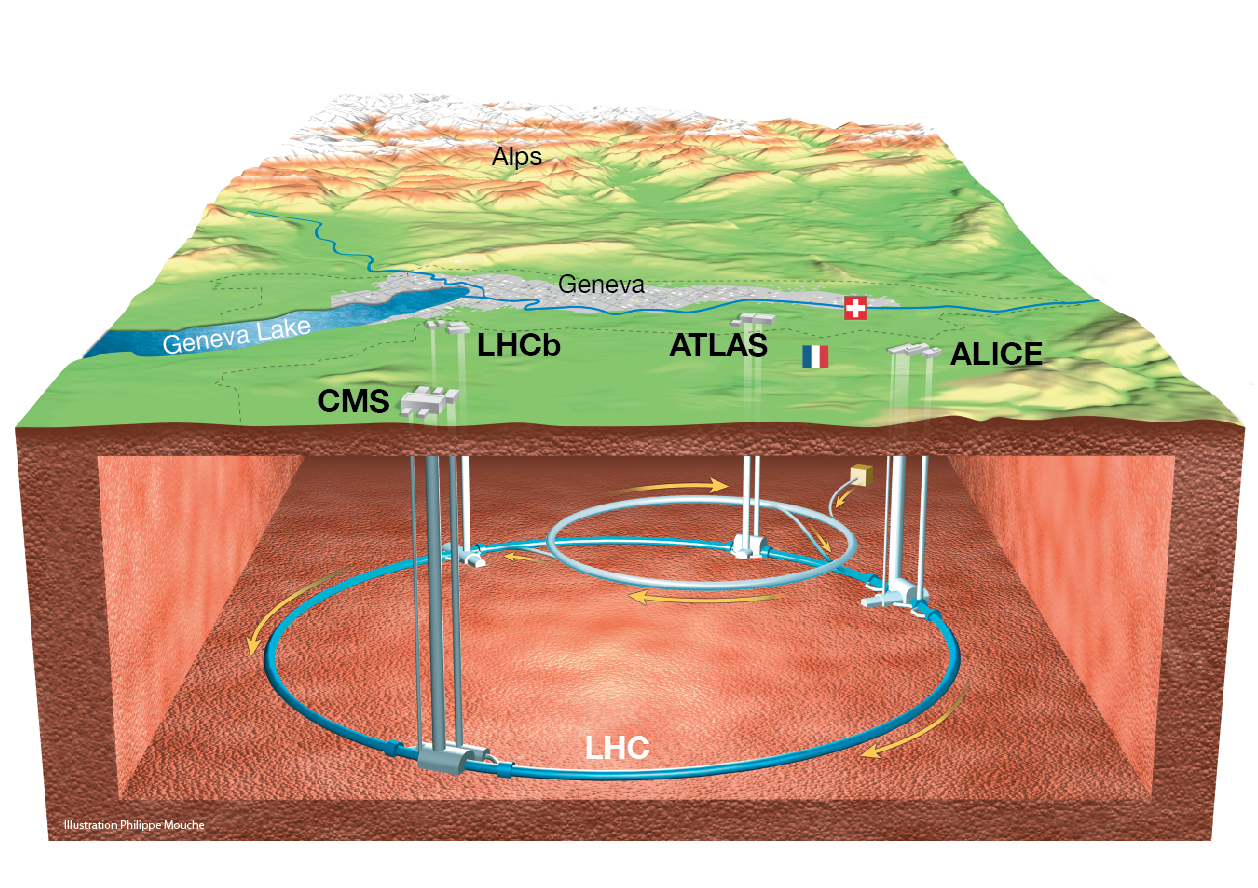
\includegraphics[width=10cm]{./figure/LHC.png}
  \caption{LHC加速器全体図器\cite{Collaboration_2008}}
  \label{fig:LHC}
\end{figure}

\section{ATLAS実験}
\label{sec:ATLAS-ex}
LHC加速器で行われている実験の1つにATLAS実験がある.ATLAS実験はLHCの4つの衝突点の1つに設置されたATLAS検出器を用いて陽子陽子衝突から$\mathrm{TeV}$スケールまでの高エネルギー物理事象を探索する実験である.2012年には,LHC実験の1つであるCMS実験と共にヒッグス粒子を発見し,標準理論の完成の大きな役割を担った.世界最高エネルギーのLHCを使ったヒッグス粒子やトップクォークといった重い粒子の精密測定はATLAS実験の重要な目的の1つである.他にも超対称性粒子などの新粒子を発見することが特に大きな目的となっている.現状の主要な成果としては,2013年3月にCMSとの結果と合わせて結論づけられたヒッグス粒子の発見が大きい.\par

\section{ATLAS検出器}
\label{sec:ATLAS}
ATLAS検出器の全体図を図\ref{fig:ATLAS}に示す.ATLAS検出器は直径25 $\mathrm{m}$,長さ44 $\mathrm{m}$の円筒形で,陽子同士の衝突点から生じる粒子を検出できる構造になっている.また,多数の検出器の複合体であり,内側から層状に,内部飛跡検出器,電磁カロリメータ,ハドロンカロリメータ,ミューオン検出器の順に配置されている.これらの複数の検出器を組み合わせることにより,粒子の追跡と識別をすることが可能になる.\par
ATLAS実験では,衝突点を原点として,ビーム軸方向にz軸,鉛直上向き方向にy軸をとり,LHC中心方向をx軸としている.また,円筒座標系として動径方向をR,z軸の正方向となす角を$\theta$,方位角$\phi$としている.$\theta$方向については,式\ref{eq:rapi}で示された擬ラピディティ$\eta$を用いて表すことが多い.

\begin{eqnarray}
  \eta = -\log \left(\tan \frac{\theta}{2} \right)
  \label{eq:rapi}
\end{eqnarray}

ATLAS検出器では,円筒形の側面部と底面部で検出器の種類,配置が異なるため,$|\eta| = 1$で2つの領域に分けられ,$|\eta| < 1$の側面部分をバレル部,$|\eta| > 1$の底面部分をエンドキャップ部と呼ぶ.

\begin{figure}[h]
\centering
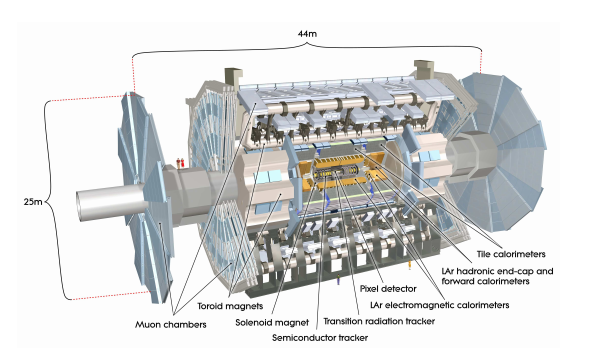
\includegraphics[width=12cm]{./figure/ATLAS.png}
\caption{ATLAS検出器全体図器\cite{Collaboration_2008}}
\label{fig:ATLAS}
\end{figure}

ATLAS検出器を構成する検出器の概要は以下のようになっている.\par
\begin{itemize}
\item 内部飛跡検出器\\
衝突点に一番近い最内層に位置する検出器,荷電粒子の飛跡を再構成して,運動量や粒子の崩壊点を測定.内側からピクセル検出器・ストリップ検出器・遷移輻射検出器で構成される.
\item 電磁カロリメータ\\
入射した電子やγ線のエネルギーおよび位置を測定.
\item ハドロンカロリメータ\\
陽子やπ中間子などのハドロンのエネルギーを測定.
\item ミューオン検出器\\
最外層に位置する検出器.ミューオンは透過率が高いため,最外層まで到達可能である.飛跡精密測定用のMonitored Drift Tube(MDT),Cathorde Strip Chamber(CSC),トリガ用のResistive Plate Chamber(RPC),Thin Gap Chamber(TGC)の4種から構成される.
\end{itemize}


\subsection{トリガシステム}
ATLAS実験では40 $\mathrm{MHz}$の頻度でバンチ衝突が起こるが,データ記録速度限界により,平均1 $\mathrm{kHz}$の頻度でしかデータを保存することができない.よって,ATLAS実験では2段階に分けたトリガシステムを導入することで興味のある事象を選び出して保存している.

\subsubsection*{Level-1 トリガ}
初段のトリガをLevel-1トリガと呼ぶ.L1トリガでは,ATLASから送られてくる40 $\mathrm{MHz}$のイベントを2.5 $\mathrm{\mu s}$以内に100 $\mathrm{kHz}$まで削減することが求められており,そのために高速処理が可能なハードウェアを用いて実行されている.\par
図\ref{fig:ATLAStrigger}にトリガの流れを示す.L1トリガは電磁カロリメータとハドロンカロリメータの情報を用いて発行されるL1Calo,ミューオン検出器の情報を用いて発行されるL1Muon,それらを組み合わせたL1Topoの3種類で構成される.\par
L1Muonはミューオン検出器のトリガ用検出器の情報を用いてトリガ判定を行う.エンドキャップ領域とバレル領域でそれぞれ独立にトリガ判定を行い,それらのトリガ情報はMuon to CTP Interface(MuCTPi)に送られ,結合される.L1CaloとL1MuonはCentral Trigger Processor(CTP)に送られると同時にTopology Processor(L1Topo)に送られる.L1TopoではL1Calo,L1Muonの情報を元に複合的なトリガを発行する.L1TopoもL1Calo,L1Muonと同じくCTPに送られ,100 $\mathrm{kHz}$に収まるように変換されたのち,L1トリガが発行される.

\begin{figure}[h]
  \centering
  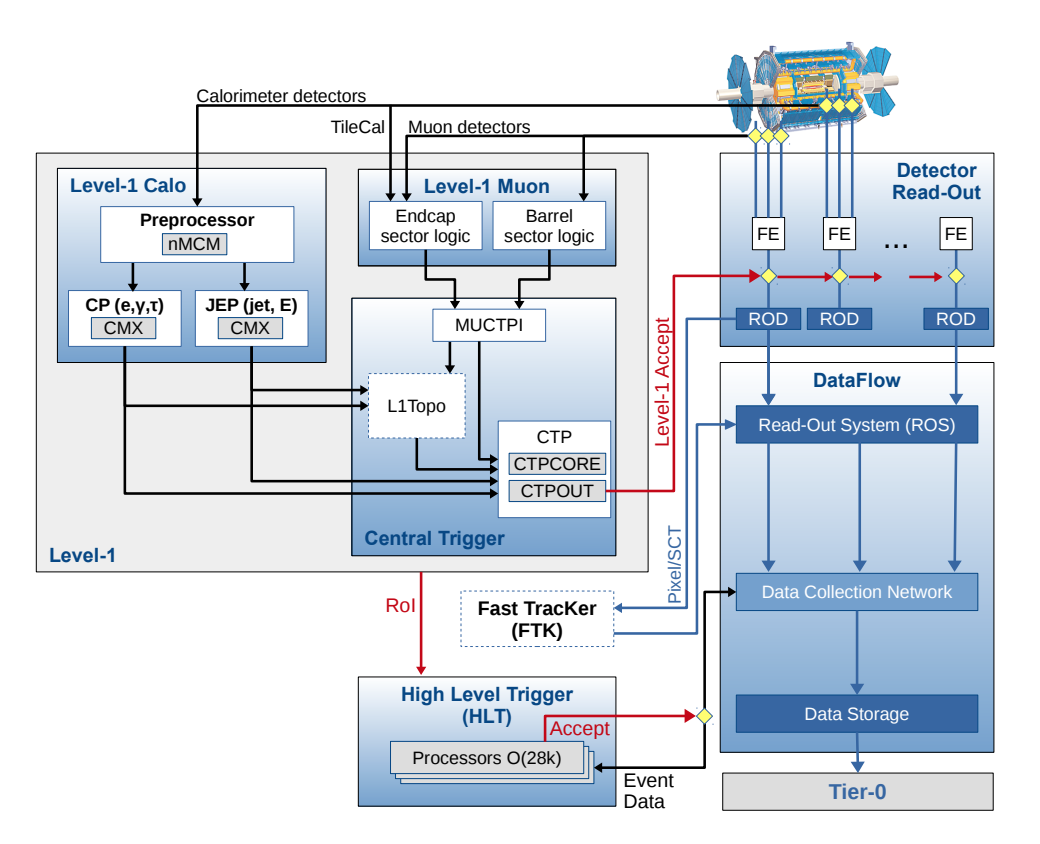
\includegraphics[width=10cm]{./figure/ATLAStrigger.png}
  \caption{ATLAS検出器のトリガの流れ\cite{Aaboud:2016leb}}
  \label{fig:ATLAStrigger}
\end{figure}


\subsubsection*{High Level Trigger}
2段目のトリガであるHigh Level Trigger(HLT)ではL1トリガを通過してイベントに対してソフトウェアを用いた高精度なトリガを発行する.内部飛跡検出器の情報を用いて荷電粒子の飛跡を再構成し,ATLAS検出器内の全ての情報を用いることでトリガレートの削減を行う.HLTは衝突から約1秒以内にイベントレートを1 $\mathrm{kHz}$まで削減し,データを保存する.

\subsection{現行の内部飛跡検出器}
現行の内部飛跡検出器は,半径1.15 $\mathrm{m}$,長さ7 $\mathrm{m}$の円筒形で,荷電粒子の飛跡を検出する.内側からInsertable B-Layer(IBL),Pixel検出器,Semiconductor Tracker(SCT)とTransition Radiation Tracker(TRT)からなり,荷電粒子の飛跡を検出する,内部飛跡検出器の構造を図\ref{fig:ID}に示す.\par
内部飛跡検出器は,衝突点で発生した荷電粒子の飛跡を検出する.それぞれの検出器からの情報を元に飛跡を再構成することによって,陽子陽子の衝突点や二次生成粒子の崩壊点の位置を測定することができる.また,外部にはソレノイド磁石があり,内部飛跡検出器全体が最大2 $\mathrm{T}$の磁場の中に配置されている.この磁場によって,荷電粒子の飛跡が曲がることから粒子の運動量を測定できる.\par

\begin{figure}[h]
  \centering
  \begin{minipage}[b]{0.45\linewidth}
    \centering
    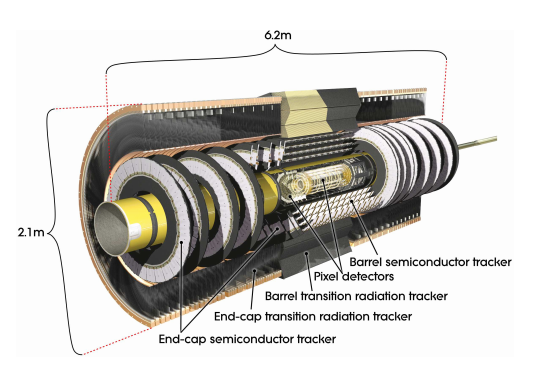
\includegraphics[width=8cm]{./figure/ID.png}
    \subcaption{全体図}
    \label{fig:ID}
  \end{minipage}
  \begin{minipage}[b]{0.45\linewidth}
    \centering
    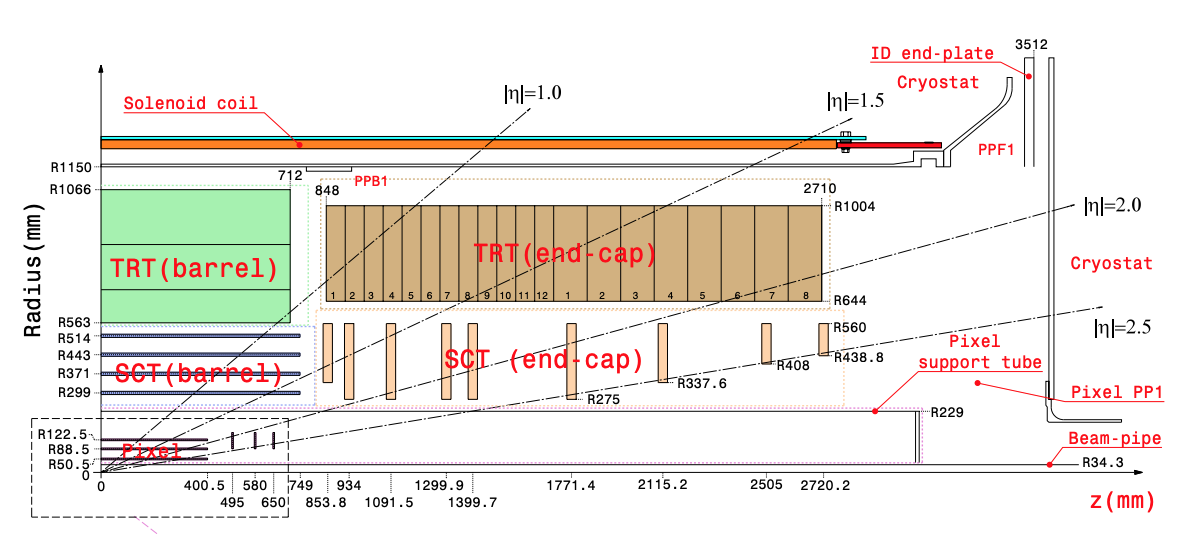
\includegraphics[width=8cm]{./figure/pixelview.png}
    \subcaption{内部飛跡検出器のレイアウト}
    \label{fig:IDview}
  \end{minipage}
  \caption{内部飛跡検出器\cite{Collaboration_2008}}
\end{figure}

\subsubsection*{Pixel検出器}
ピクセル検出器は内部飛跡検出器の最内層に位置し,バレル部3層,エンドキャップ部は片側3枚のディスクからなり,それぞれに合計約1500個,約700個の半導体検出器モジュールが配置されている.半導体検出器の仕組みについては第2章にて述べる.微小な読み出しチャンネルを2次元格子状に多数並べた作りをしているため,ピクセル検出器と呼ばれている.読み出しチャンネル毎のセンササイズが小さいため,位置分解能が高く,粒子密度の高い最内層でも粒子の飛跡の再構成の性能を維持する.2014年にバレル部最内層でとなる,Insertable B-Layer(IBL)が導入された.\par
IBL以外のピクセル検出器ははピクセルサイズが50 $\times$ 400 $\mathrm{\mu m^2}$の読み出しASIC・FE-I3を使用しており,IBLは,ピクセルサイズが50 $\times$ 250 $\mathrm{\mu m^2}$で,FE-I3と比較して放射線耐性とデータ処理速度に優れている,FE-I4と呼ばれる読み出しASICが使用されている.\par

\subsubsection*{Strip検出器}
SCTは,細長い短冊状の読み出しチャンネルを1次元方向に多数並べたストリップタイプの半導体検出器である,ストリップ間隔は80 $\mathrm{\mu m}$,長さは128 $\mathrm{mm}$である.2枚のシリコンセンサを互いに40 $\mathrm{mrad}$の角度をつけて重ねて配置し,二次元位置情報を得る.SCTの読み出しチャンネルの総数は,約630万である.

\subsubsection*{TRT}
半径24 $\mathrm{mm}$の円筒に\ce{Ar}と\ce{Xe}ガスを充填したガス検出器であり,荷電粒子の通過によって電離された電子を中心に配置されたワイヤ電極で収集する仕組みになっている.超相対論的粒子に対しては遷移輻射が起こるようになっているため,電子との識別が可能となっている.

\section{HL-LHC計画}
\label{sec:HL-LHC}
本節では,HL-LHC計画の概要とそれに伴うATLAS検出器のアップグレード項目について述べる.\par

\subsection{概要}
High Luminosity-LHC(HL-LHC)計画とは,LHCのルミノシティを向上させる計画である.これによって,統計量が増えるため,超対称性などの様々な模型が予想する新粒子への感度の向上,重い粒子の探索が可能になる.\par
HL-LHC計画に向けて,図\ref{fig:HL-LHC}のようにエネルギーやルミノシティの段階的なアップグレードが行われてきた.LHCは2010年に重心系エネルギー7 $\mathrm{TeV}$にて稼働を開始し,2010年から2013年までのデータ取得期間をRun1と呼ぶ.Run1が終わってからRun2が始まるまでの期間をLong Shutdown1 (LS1)と呼び,Run2に受けたPhase0アップグレードが行われた.Run2は2015年に重心系エネルギー13 $\mathrm{TeV}$で開始され,2018年に終了した.その後Phase1アップグレードをLS2期間に行い,2021年から2023年まで重心系エネルギー14 $\mathrm{TeV}$でのRun3が行われる予定となっている.そして,2024年から始まるLS3期間にさらなるアップグレードが行われ,2026年かあらHL-LHCとして稼働を開始する計画となっている.

\begin{figure}[h]
  \centering
  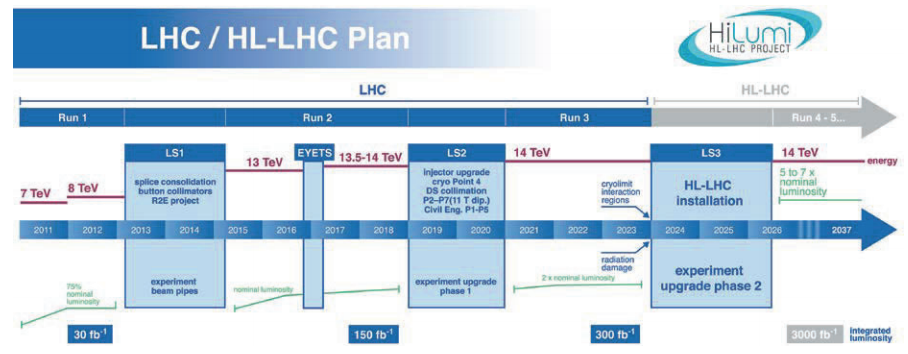
\includegraphics[width=15cm]{./figure/HL_LHC.png}
  \caption{HL-LHC計画\cite{Apollinari:2284929}}
  \label{fig:HL-LHC}
\end{figure}


\subsection{HL-LHCに伴うATLAS検出器のアップグレード}
HL-LHC計画に伴い,ATLAS検出器もアップグレードが行われる.HL-LHCを達成するために,陽子の衝突点近傍に設置する超伝導磁石や荷電粒子の飛跡を測定する内部飛跡検出器,ミューオントリガ用の電子回路の開発・製造が行われる.ATLAS検出器のアップグレードは3段階に分けて行われる.

\begin{itemize}
\item Phase0アップグレード\\
2014-2017年のLS1期間中に行われたアップグレード\\
内部飛跡検出器の最内層のピクセル検出器であるInsertable B-Layer(IBL)が導入された
\item Phase1アップグレード\\
2019-2021年のLS2期間に行われるアップグレード\\
TGCの最内層が取り替えられ,MDT,RPCでになっていた部分に新たなChamber・New Small Wheelが加えられる.また,LArトリガ回路の刷新が行われる.
\item Phase2アップグレード\\
2023-2026年のLS3期間に行われるアップグレード\\
内部飛跡検出器の総入れ替えが行われる.
\end{itemize}

\subsection{内部飛跡検出器のアップグレード}
以降,本論文に関わる内部飛跡検出器のアップグレードについて述べる.HL-LHCに向けて,内部飛跡検出器はInner Tracker(ITk)と呼ばれるシリコン検出器に置き換えられる.粒子密度の増加に対応できないためにTRT層は廃止され,内側にピクセル,それを覆うようにストリップ検出器が配置される.ピクセル検出器はバレル部とエンドキャップ部に5層,ストリップ検出器はバレル部に4層,エンドキャップ部に6層配置される予定である.図\ref{fig:ITkview}にITkのレイアウトを示す\par

\begin{figure}[h]
  \centering
  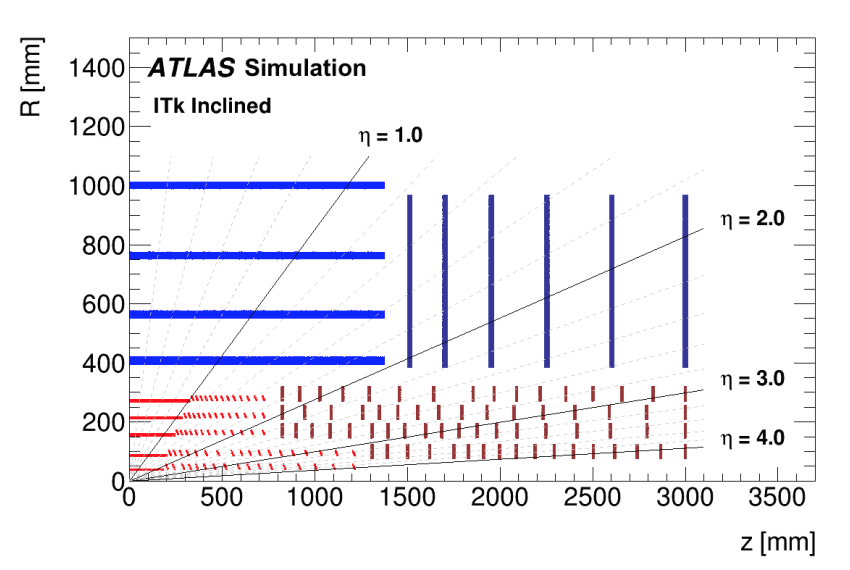
\includegraphics[width=10cm]{./figure/ITkview.png}
  \caption{Inner Trackerレイアウト\cite{Collaboration:2285585}}
  \label{fig:ITkview}
\end{figure}


現行のATLAS内部飛跡検出器は,重心系衝突エネルギー14$\mathrm{TeV}$,瞬間ルミノシティ$1 \times 10^{34} \mathrm{cm^{-2} s^{-1}}$(現在の3倍)を想定した設計になっているが,HL-LHCではビーム衝突あたりの非弾性陽子・陽子衝突の数が現在の約7.5倍に増加する.\par
この際の問題が2点存在する.1点目は,衝突あたりの生成粒子増加による放射線損傷である.ITkで想定される放射線量について,積分ルミノシティが3000 $\mathrm{fb^{-1}}$,重心系エネルギー$\sqrt{s} = 14 \mathrm{TeV}$を仮定したシミュレーションを行なった結果を図\ref{fig:radi}に示す.ここで,線量は1 $\mathrm{MeV}$の中性子に換算した,単位面積あたりの線量として表現している.最内層の放射線量は安全係数を含めて$1.4 \times 10^{16} [\mathrm{1MeV n_{eq}/cm^{2}}$]と見積もられている.検出器はこのような高い放射線に晒されることで,損傷を受けると検出効率が低下する.よって,より高い放射線耐性をもつ検出器が要求される.\par

\begin{figure}[h]
  \centering
  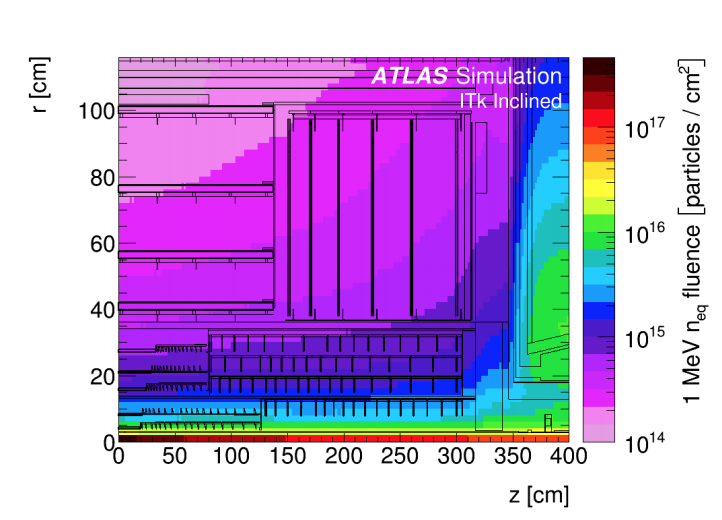
\includegraphics[width=10cm]{./figure/radi.png}
  \caption{ITkで想定される放射線量の様子\cite{Collaboration:2257755}}
  \label{fig:radi}
\end{figure}



2点目は,検出器のヒット占有率の増加である.ヒット占有率とは,衝突イベントごとに1検出器あたり,全チャンネルのうちヒット判定されたチャンネル数である,HL-LHCでは,衝突ごとに発生する粒子数が約7.5倍程度増加するため,現状の検出器のままでは,ヒットチャンネルで埋まり,パターン認識を用いた飛跡再構成の性能が低下する.HL-LHCの環境下で飛跡再構成の性能を維持したまま運転を続けるためには,より微細に位置検出が可能な検出器が必要となる.次の項目にて,これらの問題対策のためにピクセル検出器に求められるアップグレードを説明する.\par

\subsubsection*{Pixel検出器のアップグレード}
HL-LHCにおける高い放射線環境とヒット占有率の増加に対応するため,Pixelはより放射線耐性の高いもの,よりピクセルサイズが小さいものへの変更が要求される.飛跡再構成の性能を維持するために,衝突ごとに発生する粒子の密度が5倍程度増加することに合わせ,ピクセルのサイズを現行のPixelの1/5まで小さくし,チャンネル数を5倍に増やしたセンサを配置する.それにあわせて,ピクセル検出器からの信号を読み出すためのの特定用途向け集積回路(ASIC)についても現行と比べてより性能が高いものが要求される.現在はその要求を満たす新型ASICのプロトタイプ版が完成している.\par

%\subsection{アップグレードに伴うモジュールの量産}
%前節でも述べたように,HL-LHC計画に伴い,内部飛跡検出器の総入れ替えが計画されている.これにあたって,内部に用いるピクセルモジュールの量産が必要となる.そのため,世界で約10000個のモジュールの量産が計画されており,日本グループはそのうちの約2000個を担当する予定になっている.\par
%現在,新型ASICのプロトタイプ版が1チップ接続されたシングルチップモジュールが生成されており,2月ごろに4チップ接続されたクアッドチップモジュールが完成する予定である.このクアッドチップモジュールを用いて,量産体制の確認が行われ,実機で用いられる新型ASIC付きモジュールの量産に向けた体制が見直される計画である.



%LHCは2010年から運転を開始し,7TeVから8TeVの重心系エネルギーで2012年まで稼働した.この期間をLHC Run1と呼び,瞬間最高ルミノシティは$0.77\times10^{34} \mathrm{cm^{-2}s^{-1}}$であった.その後,2013年から2015年までのシャットダウン期間で加速器のアップグレードを行い,2015年からは重心系エネルギー$13\mathrm{TeV}$でLHC Run2が始まり,2018年まで続いた.Run2の3年間で得られた積分ルミノシティは約$150\mathrm{fb}^{-1}$であった.\par
%LHCは2年間のシャットダウン期間を経て2021年から重心系エネルギー$14\mathrm{TeV}$のLHC Run-3を予定している.Run-3が約3年間運転したのち,シャットダウン期間を挟んで,High Luminosity LHC(HL-LHC)が開始する予定である.
 
